\let\negmedspace\undefined
\let\negthickspace\undefined
\documentclass[journal]{IEEEtran}
\usepackage[a5paper, margin=10mm, onecolumn]{geometry}
%\usepackage{lmodern} % Ensure lmodern is loaded for pdflatex
\usepackage{tfrupee} % Include tfrupee package

\setlength{\headheight}{1cm} % Set the height of the header box
\setlength{\headsep}{0mm}     % Set the distance between the header box and the top of the text

\usepackage{gvv-book}
\usepackage{gvv}
\usepackage{cite}
\usepackage{amsmath,amssymb,amsfonts,amsthm}
\usepackage{algorithmic}
\usepackage{graphicx}
\usepackage{textcomp}
\usepackage{xcolor}
\usepackage{txfonts}
\usepackage{listings}
\usepackage{enumitem}
\usepackage{mathtools}
\usepackage{gensymb}
\usepackage{comment}
\usepackage[breaklinks=true]{hyperref}
\usepackage{tkz-euclide} 
\usepackage{listings}
% \usepackage{gvv}                                        
\def\inputGnumericTable{}                                 
\usepackage[latin1]{inputenc}                                
\usepackage{color}                                            
\usepackage{array}                                            
\usepackage{longtable}                                       
\usepackage{calc}                                             
\usepackage{multirow}                                         
\usepackage{hhline}                                           
\usepackage{ifthen}                                           
\usepackage{lscape}
\begin{document}

\bibliographystyle{IEEEtran}
\vspace{3cm}

\title{NCERT - 12.8.2.4}
\author{EE24BTECH11040 - Mandara Hosur}
% \maketitle
% \newpage
% \bigskip
{\let\newpage\relax\maketitle}

\renewcommand{\thefigure}{\theenumi}
\renewcommand{\thetable}{\theenumi}
\setlength{\intextsep}{10pt} % Space between text and floats


\numberwithin{equation}{enumi}
\numberwithin{figure}{enumi}
\renewcommand{\thetable}{\theenumi}

\textbf{Question:}\\
Using integration, find the area of region bounded by the triangle whose vertices are $\brak{-1,0}$, $\brak{1,3}$, and $\brak{3,2}$. \\

\textbf{Solution (using the trapezoidal rule):} \\
The trapezoidal rule approximates the area $A$ under a curve $y\brak{x}$ over an interval $\sbrak{a,b}$ by dividing the area to be computed into multiple trapezoids. \\

First, we define $h$. This quantity represents the width of each trapezoid (the distance between the two parallel sides of the trapezoid).
\begin{align}
h = \frac{b-a}{n}
\end{align}
Here, $n$ represents the total number of trapezoids the area to be integrated is split into. The higher the value of $n$, the smaller the value of $h$. This increases the accuracy of the computed integral. \\

The area $a_0$ of any of the trapezoids can be calculated as illustrated:
\begin{align}
a_0 = \frac{1}{2} \brak{\text{sum of lengths of parallel sides}} \brak{\text{width}} \\
\implies a_0 = \frac{1}{2} \sbrak{y\brak{x} + y\brak{x + h}} \brak{h}
\end{align}
Here, $x$ is any value in the interval $\sbrak{a,b}$. \\

Taking $a = x_0$, $b = x_n$, and defining $A_k$ as the area under the curve $y\brak{x}$ from $x = x_0$ to $x = x_k$, we can define the following relation (assume $x_{k+1} = x_k + h$ for $0<k<n$):
\begin{align}
A_{k+1} = A_k + \frac{h}{2}\brak{y_{k} + y_{k+1}} \label{area diff eq}
\end{align}

It is known that
\begin{align}
y_{k+1} = y_k + hy^{\prime}_k \label{diff eq}
\end{align}

Hence, equation \eqref{area diff eq} can be rewritten using equation \eqref{diff eq} as
\begin{align}
A_{k+1} = A_k + \frac{h}{2}\brak{2y_{k} + hy^{\prime}_k} \\
\implies A_{k+1} = A_k + hy_k + \frac{h}{2}y^{\prime}_k
\end{align}

The final sum $A_n$ gives us a good approximation of the area $A$ that we were originally attempting to compute.
\begin{align}
A = \int_{a}^{b} y\brak{x} \,dx = \frac{h}{2}\brak{y\brak{a} + 2\sum_{i=1}^{n-1}y\brak{x_i} + y\brak{b}}
\end{align}

Now, the above concept is to be implemented to find the area of the triangle mentioned in the question.
\begin{align}
A = \text{ area under } AB + \text{ area under } BC - \text{ area under } AC
\end{align}

Let the area under $AB$, $BC$, and $AC$ be $p$, $q$, and $r$, respectively. Then,
\begin{align}
A = p + q - r \label{A eq}
\end{align}

Line equation of side $AB$ can be expressed as:
\begin{align}
y = \frac{3}{2}\brak{x+1} \text{ and } y^{\prime} = \frac{3}{2}.
\end{align}

Hence area equation can be written as:
\begin{align}
A_{k+1} = A_k + h\brak{\frac{3}{2}\brak{x_k+1}} + \frac{h}{2}\brak{\frac{3}{2}}
\end{align}

Taking $x_0 = -1$ and $x_n = 1$ gives
\begin{align}
A_n = p = 3 \label{p}
\end{align}

Line equation of side $BC$ can be expressed as:
\begin{align}
y = \frac{-1}{2}\brak{x-7} \text{ and } y^{\prime} = \frac{-1}{2}.
\end{align}

Hence area equation can be written as:
\begin{align}
A_{k+1} = A_k + h\brak{\frac{-1}{2}\brak{x_k-7}} + \frac{h}{2}\brak{\frac{-1}{2}}
\end{align}

Taking $x_0 = 1$ and $x_n = 3$ gives
\begin{align}
A_n = q = 5 \label{q}
\end{align}

Line equation of side $CA$ can be expressed as:
\begin{align}
y = \frac{1}{2}\brak{x+1} \text{ and } y^{\prime} = \frac{1}{2}.
\end{align}

Hence area equation can be written as:
\begin{align}
A_{k+1} = A_k + h\brak{\frac{1}{2}\brak{x_k+1}} + \frac{h}{2}\brak{\frac{1}{2}}
\end{align}

Taking $x_0 = -1$ and $x_n = 3$ gives
\begin{align}
A_n = r = 4 \label{r}
\end{align}

Therefore the required area can be found from \eqref{A eq} as
\begin{align}
A = 3+5-4 \\
\implies A = 4 \label{numerical sol}
\end{align}

\textbf{Solution (using manual methods):} \\
Equation \eqref{A eq} can be solved using the manual method of integration, as illustrated below:
\begin{align}
A = \int^{1}_{-1} \frac{3}{2}\brak{x+1} \,dx + \int^{3}_{1} \frac{-1}{2}\brak{x-7} \,dx - \int^{3}_{-1} \frac{1}{2}\brak{x+1} \\
\implies A = \sbrak{\frac{3}{4}x^2+\frac{3}{2}x}^{1}_{-1} + \sbrak{\frac{-1}{4}x^2+\frac{7}{2}x}^{3}_{1} - \sbrak{\frac{1}{4}x^2 + \frac{1}{2}x}^{3}_{-1} \\
\implies A = 3 + 5 - 4 \\
\implies A = 4 \label{theoretical sol}
\end{align}

Clearly, from equations \eqref{numerical sol} and \eqref{theoretical sol}, we see that the area has been approximated by the trapezoidal rule well. 

\textbf{Plotting the triangle using difference equation:} \\
\begin{align}
\frac{dy}{dx} = \frac{y(x+h) - y(x)}{h} \\
\implies y(x+h) = y(x) + h\cdot\frac{dy}{dx} \label{difference equation in terms of y}
\end{align}

Let $x_0$ and $y_0$ be the initial conditions. Let some $x_1 = x_0 + h$. Then
\begin{align}
y_1 = y_0 + h\cdot\brak{\frac{dy}{dx}}_{\brak{x_0,y_0}} \label{initial difference equation}
\end{align}

Iterating through the above-mentioned process to generate $y_2$, $y_3$, $y_4$ and so on generalises equation \eqref{initial difference equation} to

\begin{align}
y_{n+1} = y_n + h\cdot\brak{\frac{dy}{dx}}_{\brak{x_n,y_n}}
\end{align}

The smaller the value of $h$, the more accurate the curve is.

For lines $AB$, $BC$, and $CA$
\begin{align}
y_{n+1} = y_n + \frac{3}{2}h \\
y_{n+1} = y_n + \frac{-1}{2}h \\
y_{n+1} = y_n + \frac{1}{2}h 
\end{align}
respectively. 

\newpage

The curve generated using method of finite differences is compared with the actual plot of the triangle in the figure below.

\begin{figure}[h]
	\centering
	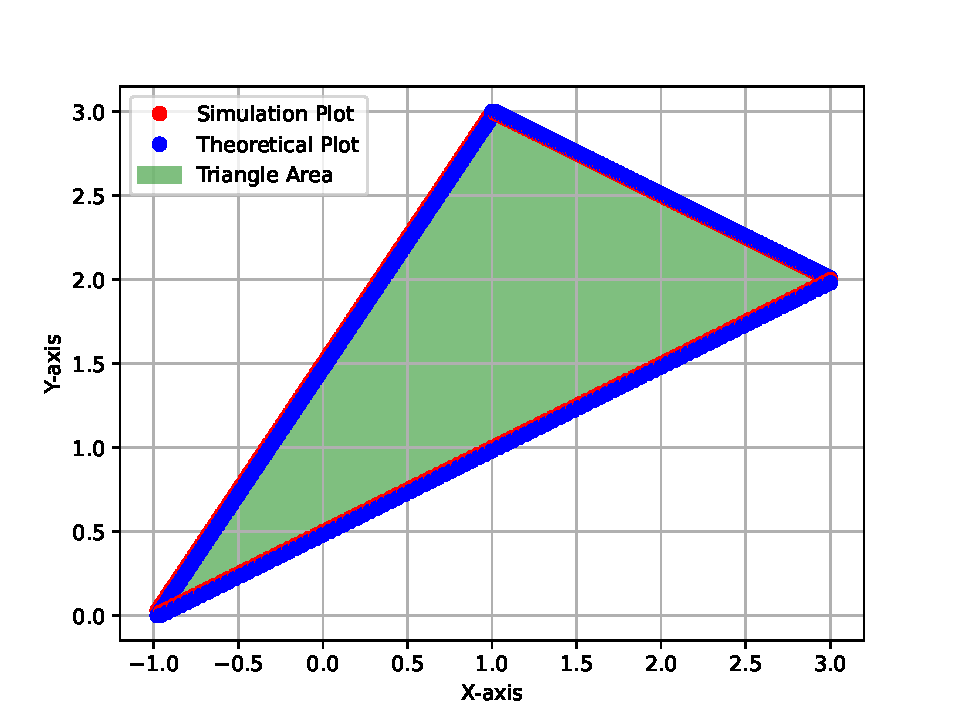
\includegraphics[width=\columnwidth]{figs/triangle.pdf}
	\caption{Plot of Given Triangle}
	\label{fig2}
\end{figure}

\end{document}
